%version of 11-26-19

\chapter{SOLUTION TO EXERCISES}
\label{ch:Exercises}


*****************

$\N_q$ is never closed under the operation of division when the modulus $q$ is composite.

\subsection{Divisibility}

Every integer $n>1$ is divisible by at least one prime number.

*****************

Prove that $f = O(g)$ and $h = O(k)$ for function $f,g,h,k$ implies that
$f+h = O(g+k)$

*****************

Prove Theorem~\ref{thm:equality=finest-equiv}

*************

For all $\langle x,y \rangle \in \N^+ \times \N^+$

$\a(x,y) \ \eqdef \ 2^{x-1} \cdot (2y -1)$

verify function $\a$'s
bijectiveness.



\section{Sets}

Define the following two operations from union and set
difference: {\it intersection} ($S \cap T$), which isolates all
elements that sets $S$ and $T$ share, and {\it symmetric difference}
($S+T$), which isolates all elements that belong to precisely one of
$S$ and $T$.


\subsection{Logic}

After consulting Fig.~\ref{fig:defns-via-tables}:

\begin{tabular}{llcl}
1. &
{\it Prove that the Propositional expression} &
$\sim P \ \Rightarrow \ P$ &
{\it is a tautology.} \\
2. &
{\it Prove that the Propositional expression} &
$P \ \Rightarrow \ \sim P$ &
{\it is satisfiable.}
\end{tabular}



*****************

Prove that when you do Euclidian division, then the {\em remainder}
upon each consecutive division is the next lowest-order digit in the
base-$b$ numeral for $n$.

******************

Prove Proposition~\ref{thm:pascal-binom} via the double induction
outlined in the text.


*******************

Complete the proof of Fig. 7.17 and similar geometric arguments: show
that all points in the areas are captured
{\Denis What is this figure?}

********************

Prove Proposition~\ref{thm:|Q|=|N|}

\noindent \textit{The problem:}
Prove $|\Q| \ = \ |\N|$.
\medskip

from Proposition~\ref{thm:|NxN|=|N|}.


*********************

Prove that the views of SAT are equivalent: (1) a set of clauses; (2)
a disjunction of clauses.


**********************

\subsection{Link of equality and equivalence relation}
Application

\noindent \textit{The problem:}
The equality relation, $=$, on a set $S$ is the {\em finest}
equivalence relation on $S$, in the sense that $=$ refines every
equivalence relation on $S$.
\medskip

*********************

\textbf{ Play} with negating strong (weak) relations to get weak (strong) ones.
 


*********************

 The biggest and smallest elements of
${\cal P}(S)$ are, respectively, the set $S$ itself and the empty set
$\emptyset$.

\subsection{Revisiting a very old problem}

\noindent \textit{The aim:}
To write
\medskip

\noindent \textit{The problem:}

{\Arny Because your geometric solution below involves just a single
  special quadratic --- and one that seems not to have other special
  interest --- I propose that we include it in some form of ENRICHMENT
  section.  }

{\ignore {\Denis It is interesting here to stress how hard it was to solve such equations. Algebra raised only in the second half of the last millenium.
However, there are several nice examples of geometrical solutions.
One of the oldest comes from babylonians in the 18th century BC.
The numeral system was in base 60, and the problem was to determine the length of the side of a square which was part of a larger rectangle.
The following figure details the process.}}

\begin{figure}[htb]
\begin{center}
       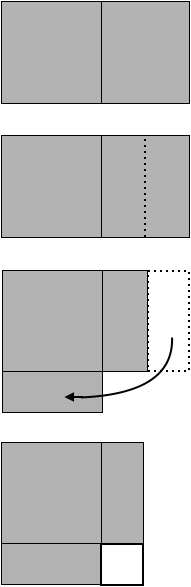
\includegraphics[scale=0.4]{FiguresArithmetic/tabletteMesopotamie}
\caption{Solving $x^2 + x = 45$.
The idea of the proof is to represent the left hand side by the square $x^2$ beside a rectangle $60 \times x$.
Then, split the right rectangle into two equal parts and move one part a the bottom of the left square.
The final figure shows the whole square whose surface is equal to $45$ plus the surface of the white square
whose surface is equal to $30 \times 30$.
In base $60$, this is $15$. 
$45+15 = 60$, thus, the big square is the unit square, its side is $60$.
Thus, the length of the initial square is equal to $60-30=30$.}
\label{fig:equationBabillon}
\end{center}
\end{figure}


%%%%%%%%%%%%%%%%%%%%%%%%%%%%%%%%%%%%%%%%%%%

\section{Summations}



\subsection{Compute $\Delta_n$ by means of sum of squares}

$\Delta_n = \sum_{i=1}^{n} i = \frac{n(n+1)}{2}$

The idea here is to write the sum by extracting the first and the last element
of the sum of squares.
%We loose since the coefficient of the $\Delta_n$ is the same after these manipulations, but we can manage if we compute the \textit{next} sum, that is sum of the squares.
\medskip

$S_{n+1} = 1 + \sum_{i=1}^{n+1} i^2$

$S_{n+1} = (\sum_{i=1}^{n} i^2) + (n+1)^2$

where $\sum_{i=1}^{n+1} i^2 
= \sum_{i=0}^{n} (i-1)^2 
= \sum_{i=0}^{n} (i^2-2i+1) 
= \sum_{i=0}^{n} i^2- 2 ( \sum_{i=0}^{n} i) + (n+1)
= \sum_{i=1}^{n} i^2- 2 ( \sum_{i=1}^{n} i) + (n+1)$

Thus, 
$\sum_{i=1}^{n} i^2- 2 ( \sum_{i=1}^{n} i) + (n+1) = (\sum_{i=1}^{n} i^2) + (n+1)^2$

$-2 \Delta_n + (n+1) =  (n+1)^2$

$\Delta_n =  (n+1)^2-(n+1) = n(n+1)$



\subsection{Training on undetermined coefficient method}

\noindent \textit{The problem.}
Say that you are told that the sum of the first $n$ perfect squares is
a {\em cubic} polynomial in $n$.  Use the method of undetermined
coefficients to derive the exact formula (\ref{eq:sum-1-to-nsq1}) for
the sum.
\medskip

\noindent \textit{The solution.}

to be done


\subsection{Tetrahedral numbers}

\noindent \textit{The aim.}
$\Theta_n$ is defined as the sum of the triangular numbers $\Delta_n$:

$\Theta_n =  \sum_{k=1}^{n} \Delta_k$

Our objective here is to give an expression of these numbers.
\medskip

\noindent \textit{The problem.}
Prove the following expression

$\Theta_n = \frac{n.(n+1).(n+2)}{6}$
\medskip

\noindent \textit{Hint.}
This result can easily been proved by recurrence, we let the reader develop it. 
We suggest to use the double counting Funini's principle.

Following this way, you should write the previous expression of the tetrahedral number in a developed form 
using a triangle shape as shown in Fig.~\ref{fig:TetrahedralBasic}.
\begin{figure}[h]
\begin{center}
        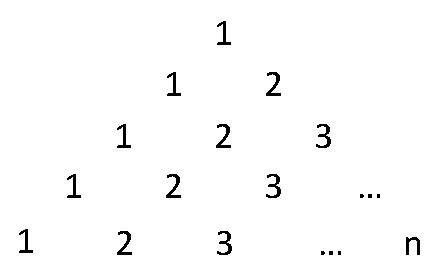
\includegraphics[scale=0.5]{FiguresArithmetic/TetrahedralBasic}
        \caption{Computing $\Theta_n$: basic triangle pattern.}
        \label{fig:TetrahedralBasic}
\end{center}
\end{figure}
and draw two copies by rotating the dimensions.

Fubini's principle is used by summing up the successive rows.

Prove as an intermediate result that the sum of the elements over the rows of the three triangles is proportional to $n+2$.
\medskip

\noindent \textit{The detailed solution.}
We proved the expression of $\Delta_n$ by mirroring the developed expression and adding term by term.
Similarly, a way to prove the expression of $\Theta_n$ is to consider three copies and organize them 
in order to obtain the expected result.
A tetrahedral number can be arranged as a triangle (see Fig.~\ref{fig:TetrahedralBasic}).
%\begin{figure}[h]
%\begin{center}
%        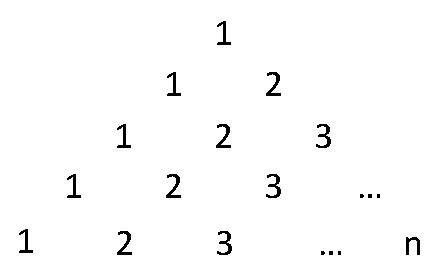
\includegraphics[scale=0.5]{FiguresArithmetic/TetrahedralBasic}
%        \caption{Computing $\Theta_n$: basic triangle pattern.}
%        \label{fig:TetrahedralBasic}
%\end{center}
%\end{figure}

The proof is obtained by the double counting principle by rotating the three faces of triangles as shown in Fig.~\ref{fig:Tetrahedral}.
\begin{figure}[h]
\begin{center}
        \includegraphics[scale=0.5]{FiguresArithmetic/Tetrahedral}
        \caption{Computing $\Theta_n$ using an adequate arrangement of $3$ triangles.}
        \label{fig:Tetrahedral}
\end{center}
\end{figure}

Sum up all the numbers in each row.

\begin{itemize}
\item 
The first row is equal to $1+1+n = n+2$.
\item
The second one is equal to $3 + 3 + 2(n-1) = 2(n+2)$. 
\item
Let us sum up the elements in row $k$: 

$\Delta_k + \Delta_k + k(n-k+1)  = k(k+1) + kn-k^2+k = k(n+2)$.
\end{itemize}

Conclusion:
the global sum is equal to $n+2$ times $(1+2+...+n)$.

Finally, $3 \Theta_n = (n+2) \Delta_n$.
\medskip

\noindent \textit{Going further.}

Summary: we proved the following results:
\begin{itemize}
\item $Id_n = 1+1+ ... +1 = n$
\item $\Delta_n = 1+2+3+ ... +n = \frac{1}{2}.Id_n.(n+1)$
\item $\Theta_n = \Delta_1 + \Delta_2 + ... + \Delta_n = \frac{1}{3} .\Delta_n.(n+2)$
\end{itemize}

A natural question is if we can go further following the same pattern for computing 
$ \sum_{k=1}^{n} \Theta_k$, and so on.

Are you able to consider the challenge?


\subsection{Sum of perfect cubes}

\noindent \textit{The aim:}
This exercice presents an alternative proof of the result of Section~\ref{sec:sumOfOdds},
that establishes that the sum of $n$ first cubes is equal to a perfect square.
\medskip

\noindent \textit{The problem.}
Show that the sum of $n$ first cubes is equal to a perfect square, and more precisely, $\Delta_n^2$.
\medskip

\noindent \textit{The solution.}
The proof is based on an hold and simple pattern that we learned in elementary school.
\medskip

\index{$n^2$ as sum of first $n$ odd integers!a proof from elementary school}
\begin{proof}
%
Consider the following reasoning which emerges from the way
multiplication tables are developed in elementary school.  
Let us first illustrate the idea using the case $n=5$.
\begin{equation}
\label{eq:Fubini-table}
\begin{array}{rrrrr}
1  &  2 &  3 &  4 &  5 \\
2  &  4 &  6 &  8 & 10 \\
3  &  6 &  9 & 12 & 15 \\
4  &  8 & 12 & 16 & 20 \\
5  & 10 & 15 & 20 & 25 \\
\end{array}
\end{equation}
Write the integers $1, 2, \ldots, n$ in a row.  Below this row, write
the doubles of these integers.  Below the ``double'' row, write the
triples of the integers.  Below the ``triple'' row, write the
quadruples of the integers, then the quintuples, and so on.  Note that
the resulting table is {\em symmetric:} its rows are identical to its
columns.
\medskip

Using again Fubini's rearrangement stratagem, we now count all the integers in
the table in two different ways.
\begin{enumerate}
\item
We sum the entries of our table by peeling away successively larger
reversed instances of the letter ``$L$'' (as in our earlier
``pictorial'' proof of
Proposition~\ref{thm:squares-odd-integers-Gauss}).  We find that the
integers in each ``$L$'' sum to a perfect cube.
Actually, the diagonal is (by definition) equals to the square.
\[
\begin{array}{rrrrrrrrr|rrc}
1  &    &    &    &    &   &     &    &   & 1   & = 1^3 \\
2  &  4 &  2 &    &    &   &     &    &   & 8   & = 2^3 \\
3  &  6 &  9 &  6 &  3 &   &     &    &   & 27  & = 3^3 \\
4  &  8 & 12 & 16 & 12 &  8 &  4 &    &   & 64  & = 4^3 \\
5  & 10 & 15 & 20 & 25 & 20 & 15 & 10 & 5 & 125 & = 5^3
\end{array}
\]

\item
We sum the successive rows of the $n \times n$ table (\ref{eq:Fubini-table}).  
The first row of the table sums to $\Delta_n$; the second row sums to $2
\Delta_n$; the third row sums to $3 \Delta_n$; \ldots; the last row sums
to $n \Delta_n$.  
Thus, the aggregate sum of the table's rows is 
\[ (1 + 2 + \cdots + n) \cdot \Delta_n \ = \ \left(\Delta_n \right)^2 \]
\end{enumerate}
We conclude that
\[
\sum_{i=1}^n i^3 \ = \  \left(\Delta_n \right)^2
\]
\end{proof}


\subsection{Harmonic series}

\noindent \textit{The aim.}
Show another way to prove that the sum of harmonic terms $H_{n} = \sum_{k=1}^{n} \frac{1}{k}$ is infinite.
\medskip

\noindent \textit{The problem}

Show that the harmonic series diverges (it goes to infinity).
\medskip

\noindent \textit{Hint.}
Group the terms of the series in an adequate way.
\medskip

 \noindent \textit{The solution.}
The analysis is as follows.

A first solution is to group the terms according to powers of $2$. 
Then, the sum within each group is between $\frac{1}{2}$ and $1$, thus,
$H_n > \frac{1}{2}.n$
\medskip

Another (more precise) way is to gather the terms 3 by 3 as follows:

$S_k = (\frac{1}{3k-1} + \frac{1}{3k} + \frac{1}{3k+1} )$ for $k\geq1$, 

$H = 1 + S_1 + ... + S_k + ... > 1 + 3.\frac{1}{3} + 3.\frac{1}{6} + ... + 3.\frac{1}{3k} + ... $

since $S_k > 3.\frac{1}{k} $.

The proof is by contradiction:

if $H$ is finite, from the previous relation we have: $H > 1 + H$, which is obviously impossible.
\medskip

Moreover, the first way of  bounding the sum tells us about its value (actually, we know the value at a factor of $2$):

$\frac{log(n)+1}{2} < H_n < log(n)+1$. Thus, $H_n = O(log(n))$


%%%%%%%%%%%%%%%%%%%%%%%%%%%%%%%%%%


\section{Proof techniques}


\subsection{On meeting new people}

\noindent \textit{The aim.}
Illustration of pigeon's hole principle.
\medskip

\noindent \textit{The problem.}
You are attending a cocktail party that is populated by $n$ couples.
In order to create a warm atmosphere, the host requests that each
attendee shake the hand of every attendee that he or she does not
know. \\
Prove that some two attendees shake the same number of hands.
\medskip

\noindent \textit{The solution.}
%
This observation follows from the \textit{pigeonhole principle}:
If $n+1$ pigeons occupy $n$ pigeonholes, then some hole contains
at least $2$ pigeons.
{\Denis is it useful to recall the principle here? I don't think so...}

This principle guarantees that some two attendees shake the same
number of hands.  To wit, the number of people that each attendee {\em
  does not know} belongs to the set $\{ 0, 1, \ldots, 2n-2 \}$,
because each person knows him/herself and his/her partner.  Because
there are $2n$ handshakers (the pigeons) and $2n-1$ numbers of hands
to shake (the boxes), some two shakers must shake the same numbers of
hands. 
\medskip

\noindent \textit{Lesson learned.}
Training for mastering different types of proofs, here the focus is put on Pigeonhole.


%%%%%%%%%%%%%%%%%%%%%%%%%%%%%%%%%%%%%%%

\section{Graphical proofs}

\subsection{A graphical proof for a specific geometric series}

\noindent \textit{The aim.}
To develop more intuition in solving using geometrical arguments.

Particular case of geometric series.
\medskip

\noindent \textit{The problem.}
Compute the sum of $(\frac{1}{4})^k$ using a graphical argument ($k \geq 0$).
\medskip

\noindent \textit{The solution.}
A rapid analysis of the small values of $k$ leads to the guess $(\frac{1}{4})^k = \frac{1}{3}$.
 
The solution is depicted in Fig.~\ref{Fig:SUmgeo1sur4}. 
\begin{figure}
\begin{center}
        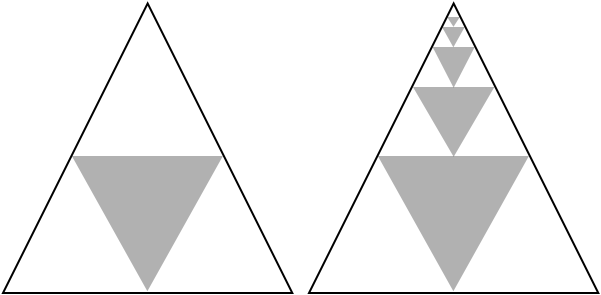
\includegraphics[scale=0.3]{FiguresArithmetic/SumGeometric1sur4}
        \caption{Graphical construction. Assuming the total area is 1, the area of the grey internal triangle (left) is $\frac{1}{4}$.
        As the grey area is one third at each layer (right), the whole area is $\frac{1}{3}$.
        By the double counting Fubini's principle, this area is the sum of the $\frac{1}{4^k}$ (for $k \geq 1$).}
        \label{Fig:SUmgeo1sur4}
\end{center}
\end{figure}

Finding such a triangular pattern may not be considered as an easy task.
However, as stated in the problem, the main point is to divide an elementary surface
into four equal pieces. 
Squares (or even worse disks) are not simple to use in this context while equilateral triangles 
are a \textit{natural} structure. 
\medskip

\noindent \textit{Lesson learned.}
Training and gain intuition for mastering geometrical proofs. 


\subsection{A graphical proof}

\noindent \textit{The aim.}

Use a pictural argument to prove a nonobvious identity of arithmetic sums
that one would be unlikely to come upon by purely textual thinking.
\medskip

\noindent \textit{The problem.}
\begin{prop} 
\label{thm:an-arithmetic-identity}
For any positive integer $n$,
\[ \Delta_{2n-1} \ = \ n + 4 \Delta_{n-1}. \]
\end{prop} 
\medskip

\noindent \textit{The solution.}
\begin{proof} 
Consider the arithmetic series in (\ref{eq:arith-seq}) for the case
$a=1$ and $b=4$.  
By Proposition~\ref{thm:sum-of-arithmetic-series},
this series, call it $S^{(1,4)}(n)$, has the sum
\begin{equation}
\label{eq:triangles}
S^{(1,4)}(n) \ = \ n + 4 \Delta_{n-1}.
\end{equation}

Let us represent the sum $\Delta_{n-1}$ in the natural way as a
triangle of tokens.  This triangle has a base of $n-1$ tokens, upon
which sits a row of $n-2$ tokens, upon which sits a row of $n-3$
tokens, \ldots, all the way to the apex, which has a single token.

Now, let us view equation (\ref{eq:triangles}) as giving us access to four
copies of the preceding triangle of tokens.  Let us arrange these
triangles in the manner depicted in Fig.~\ref{fig:Delta(n)4}.
\begin{figure}[ht]
\begin{center}
       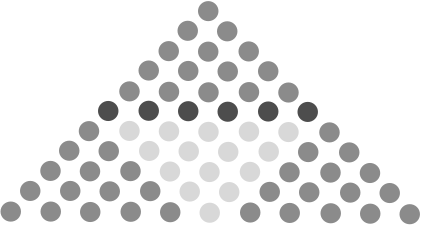
\includegraphics[scale=0.5]{FiguresMaths/Delta4}
 \caption{Arranging the four triangles plus a row to obtain a new (bigger) triangle.}
       \label{fig:Delta(n)4}
\end{center}
\end{figure}
Now, ``complete the picture'' by adding an ``extra'' row of $n$
tokens at row $n$ of the figure (these are depicted in dark gray in
the figure).  The four small triangles, augmented by the ``extra'' row
of $n$ tokens has clearly become a representation  of $\Delta_{2n-1}$
by tokens.

We now have a purely pictorial proof of the proposition. 
\end{proof} 
\medskip

\noindent \textit{Lesson learned.}

Training.


\subsection{A variant for computing $\Delta_n$}

\noindent \textit{The aim.}

Application of geometric sum.
\medskip

\noindent \textit{The problem.}

%Compute the sum of the first integers $\Delta_n$. 
Show graphically that $\Delta_n$ (sum of the first $n$ integers) is congruent to $1$ modulo $8$.
\medskip

\noindent \textit{Hint.}
Write the previous relation as $8 \Delta_n = K^2 -1$
for an integer $K$ to determine and represent the square $K$ by $K$. 

\noindent \textit{The solution.}

The expression $8 \Delta_n = (2n-1)^2 -1$ can be represented as in~\ref{fig:Sum8deltas}.
\begin{figure}[ht]
\begin{center}
       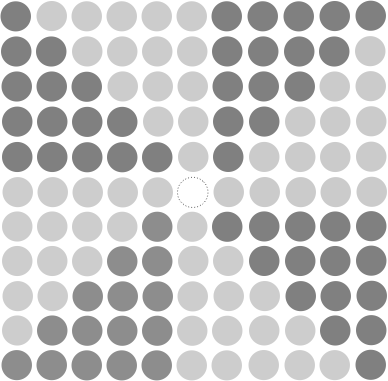
\includegraphics[scale=0.4]{FiguresMaths/Delta8}
\caption{8 copies of $\Delta_n$ are filling a big square but one token.}
       \label{fig:Sum8deltas}
\end{center}
\end{figure}



\subsection{Another proof for irrationality of $\sqrt{2}$}

\noindent \textit{The aim.}

reenforcing the ability of using geometrical proofs.
\medskip

\noindent \textit{The problem.}
Prove the irrationality of $\sqrt{2}$ using a geometrical argument.
\medskip

\noindent \textit{Hint.}
The proof is by contradiction. 

Consider $\sqrt{2}$ is rational, which means there exists a pair of integers $(a,b)$
such that $\sqrt{2} = \frac{a}{b}$ (where $a$ is larger than $b$).
Among all possible pairs, take the unique irreductible ratio.

Represent this expression geometrically by the corresponding isocele right triangle
which is the one of minimal surface. 

The contradiction comes by constructing another isocele triangle with a smaller surface.
%Squaring this expression leads to $2.b^2 = a^2$.
\medskip

\noindent \textit{The solution.}

The solution is depicted in Fig.~\ref{Fig:sqrtbisInit} and~\ref{Fig:sqrtbisFin} . 
\begin{figure}
\begin{center}
        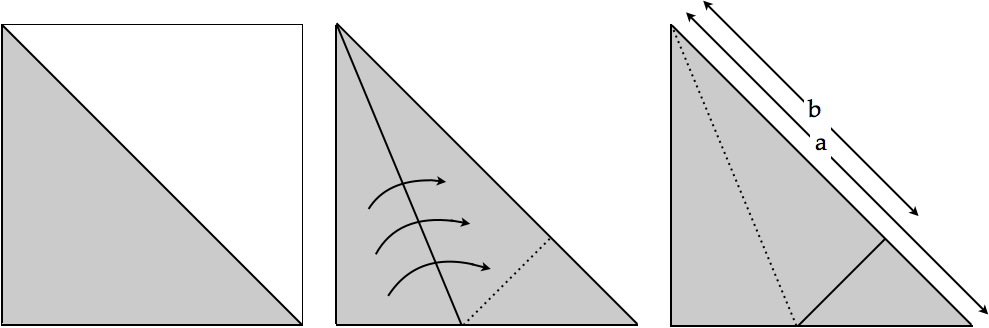
\includegraphics[scale=0.3]{FiguresArithmetic/sqrtbisInit}
        \caption{First step: folding the triangle along the side.}
        \label{Fig:sqrtbisInit}
\end{center}
\end{figure}
\begin{figure}
\begin{center}
        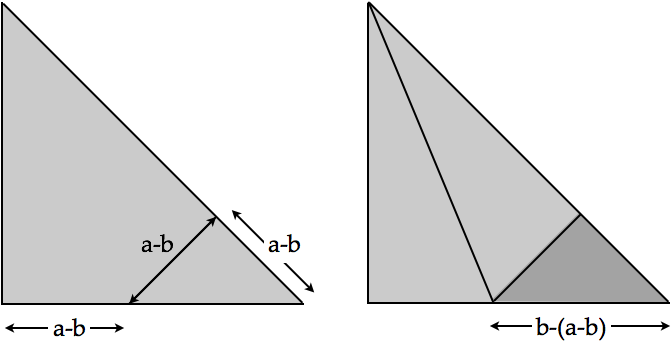
\includegraphics[scale=0.3]{FiguresArithmetic/sqrtbisFin}
        \caption{Second step. The sides of the small isocele triangle are integers.}
        \label{Fig:sqrtbisFin}
\end{center}
\end{figure}



%%%%%%%%%%%%%%%%%%%%%%%%%%%%%%%%

\section{Arithmetic}

\subsection{Complex
  multiplication via $3$ real multiplications}
\index{complex number!multiplication via 3 real multiplications}

\noindent {\it The aim.}
To be completed...
\medskip

\noindent {\it The problem.}
%\label{thm:complex-mult-3real}
Show how to compute the product of two complex numbers using only {\em three}
real multiplications rather than four.
\medskip

\noindent {\it The solution.}
Although implementing (\ref{eq:complex-mult}) ``directly'' correctly
produces the product $\kappa = (a+bi) \cdot (c+di)$, there is another
implementation that is {\em more efficient}.  Specifically, the
following recipe computes $\kappa$ using only {\em three} real
multiplications instead of the four real multiplications of the
``direct'' implementation.  We begin to search for this recipe by
noting that our immediate goal is to compute both Re$(\kappa) = ac-bd$
and Im$(\kappa) = ad+bc$.  We can accomplish this by computing the
{\em three} real products
\begin{equation}
\label{eq:complex-mult-3a}
(a+b) \cdot (c+d); \ \ \ \ \
ac;  \ \ \ \ \ bd
\end{equation}
and then noting that
\begin{equation}
\label{eq:complex-mult-3b}
\begin{array}{lcl}
\mbox{Im}(\kappa) & = & (a+b) \cdot (c+d) - ac -bd, \\
\mbox{Re}(\kappa) & = & ac -bd
\end{array}
\end{equation}
We thereby achieve the result of the complex multiplication described
in (\ref{eq:complex-mult}) while using only {\em three} real
multiplications.
\medskip

\noindent {\it Lesson learned.}

Of course, a full reckoning of the costs of the two implementations we
have discussed exposes the fact that the implementation that invokes
(\ref{eq:complex-mult-3a}) and (\ref{eq:complex-mult-3b}) uses {\em
  three} real additions rather than the {\em two} real additions of
the ``direct'' implementation.  But this entire exercise was
predicated on the observation that each real addition is much less
costly than a real multiplication, so trading one multiplication for
one addition is an unqualified ``win''. 

{\Denis do the link with Karatzuba?}


\subsection{A fun result dealing with divisibility}

\noindent \textit{The aim:}
mixed technique between divisibility and pigeon holes.

This exercice was a favorite question by Paul Erdos,
he often used this question to test the ability of young students in mathematics. 
\medskip

\noindent \textit{The problem:}
Let consider the $2n$ first integers.

Take any $n+1$ integers in this set and prove that there exists a pair $(p,q)$
such that $p$ divides $q$. 
\medskip

\noindent \textit{Hint:}

Let $\alpha_i$ be the elements of this set of cardinality $n+1$...
Write $\alpha_i = 2^k \times m$ where $m$ is odd (and $k \geq 0$).
\medskip

\noindent \textit{The detailed solution:}

%The sketch of the proof is as follows.
\begin{enumerate}
\item
Let $\alpha_i$ be the elements of this set of cardinality $n+1$.

Write $\alpha_i = 2^k \times m$ where $m$ is odd (and $k \geq 0$).

Then, $m$ belongs to $\{1,3,5, \ldots, 2n-1 \}$
\item
From the pigeon hole principle, there are two numbers with the same value of $m$. 
\item 
Thus, $2^{k1} \times m$ and $2^{k2} \times m$

$p$ is the smallest one, which divides $q$ (the largest one).
\end{enumerate}


\subsection{A ``trick'' for squaring certain integers}

Sometimes only basic knowledge is needed to craft amusing
``tricks''---we know that they are not really tricks at all!---that
are really rigorous applications of principles that we have learned.
Here is an ``old chestnut'' example that may inspire you to design
your own. 

If someone presents you with a number that has a numeral that ends in
$5$, then there is a simple way to square the number mentally.  For
instance, if someone says

\hspace{.25in}``$n = 25$''

\noindent
then you can instantly respond

\hspace{.25in}``$n^2 = 625$''

\noindent
If the challenge is

\hspace{.25in}``$n = 75$''

\noindent
then your response is

\hspace{.25in}``$n^2 = 5625$''

\noindent
Let's make this ``game'' mathematical.
\medskip


\noindent \textit{The problem:}

Let $n$ be any number that has a $2$-digit decimal numeral of the form

\hspace{.25in}$\delta \ 5$ \ \ \ \ $(\delta \in \{ 0,1,2,3,4,5,6,7,8,9\})$.

\noindent
Then the square of $n$ is the integer

\hspace{.25in}$25 \ + \ \delta \cdot (\delta +1)$. 
\medskip

\noindent \textit{The solution:}

We can rewrite the premise of the proposition in the form
\[ n \ = \ 10 \cdot \delta + 5 \]
It is now easy to invoke Proposition~\ref{prop:(a+b)(c+d)} and the
distributive law to compute that

\[ n^2 \ = \ 100 \cdot \delta \cdot (\delta+1) + 25. \]
To wit: 
\[
\begin{array}{lclll}
n^2 & = & (10 \cdot \delta + 5)^2 & & \mbox{Given} \\
    & = & 100 \cdot \delta^2 \ + \ 100 \cdot \delta \ + \ 25
              & & \mbox{the proposition} \\
    & = & 100 \cdot (\delta^2 \ + \ \delta) \ + \ 25
              & & \mbox{factoring: distributive law} \\
    & = & 100 \cdot \delta \cdot (\delta + 1) \ + \ 25
              & & \mbox{factoring: distributive law} \\
\end{array}
\]
A parlor trick has become a mathematical demonstration!
\qed
\medskip

\noindent \textit{Lesson learned}



\subsection{When is integer $n$ divisible by $9$?}
\label{sec:divisible-by-9}

\noindent \textit{The aim.}

We exploit here our ability to evaluate geometric summations to
illustrate a somewhat surprising, nontrivial fact.  One can deduce
information about the divisibility of an integer $n$ from $n$'s
positional numerals.  We hope that this ``fun'' result will inspire
the reader to seek kindred numeral-encoded properties of numbers.

\medskip
\noindent \textit{The problem.}
%\label{thm:div-by-b-bar}
An integer $n$ is divisible by an integer $m$ if, and only if, $m$
divides the sum of the digits in the base-$(m+1)$ numeral for $n$.
\medskip

The most familiar instance of this result is phrased in terms of our
traditional use of base-$10$ (decimal) numerals. \\
{\it An integer $n$ is divisible by $9$ if, and only if, the sum of
  the digits of $n$'s base-$10$ numeral is divisible by $9$.}
\medskip

\noindent \textit{The solution.}

({\it Argument for general number-base $b$}).
%
Of course, we lose no generality by focusing on numerals without
leading $0$'s, because leading $0$'s do not alter a numeral's sum of
digits.

Let us focus on the base-$b$ numeral for a number $n$ (so $b = m+1$ in
the statement of the proposition).  There therefore exist base-$b$
digits---i.e., integers from the set $\{0, 1, \ldots, b-1\}$---call
them $\delta_k \neq 0$, $\delta_{k-1}$, \ldots $\delta_1$, $\delta_0$,
such that
\[ n \ = \ \delta_k \cdot b^k + \delta_{k-1} \cdot b_{k-1} + \cdots +
\delta_1 \cdot b + \delta_0. \]
The sum of the digits of $n$'s base-$b$ numeral is, then
\[ s_b(n) \ \eqdef \ \delta_k + \delta_{k-1} + \cdots + \delta_1 +
\delta_0. \]
Let us calculate the difference $n - s_b(n)$ in the following manner,
digit by digit.
\begin{equation}
\label{eq:sum-of-digits}
\begin{array}{ccccccccccc}
n & = &
\delta_k \cdot b^k & + & \delta_{k-1} \cdot b^{k-1} & + & \cdots
  & + & \delta_1 \cdot b & + & \delta_0 \\
s_b(n) & = &
\delta_k & + & \delta_{k-1} & + & \cdots & + & \delta_1 & + & \delta_0 \\
\hline
n - s_b(n) & = &
\delta_k \cdot (b^k -1) & + &
\delta_{k-1} \cdot (b^{k-1} -1) & + &
\cdots & + &
\delta_1 \cdot (b-1) & & 
\end{array}
\end{equation}

We now revisit summation (\ref{eq:geom-sum:b>1}).  Because $b$ is a
positive integer, so that $1 + b + \cdots + b^{a-2} + b^{a-1}$ is also
a positive integer, we infer that {\em the integer $b^a -1$ is
  divisible by $b-1$.}

We are almost home.  

Look at the equation for $n - s_b(n)$ in the
system (\ref{eq:sum-of-digits}).  As we have just seen, every term on
the righthand side of that equation is divisible by $b-1$.  It follows
therefore, that the lefthand expression, $n - s_b(n)$, is also
divisible by $b-1$.
An easy calculation, which we leave to the reader, now shows that this
final fact means that $n$ is divisible by $b-1$ if, and only if, $s_b(n)$ is.
\medskip

\noindent \textit{The lesson learned.}

To be completed.


%%%%%%%%%%%%%%%%%%%%%%%%%%%%%%%%%%

\section{Combinatorics}

\subsection{Going further in a game analysis}

\noindent \textit{The problem:}
Analyze the game of craps in the same way as we did for sum-of-three

Verify the table in Fig.~\ref{fig:dice-ordered-configs}

In the ordered version of sum-of-three, sum$k$ is engendered by the
same number of configurations as is sum $21 - k$.  
Why is this the case?

\noindent \textit{The solution:}

\subsection{more about the Birthday paradox}

\noindent \textit{The aim:}
An interesting variant of the birthday puzzle
\medskip

\noindent \textit{The problem:}
Determine the
probability of a student to be born the same day as me.
\medskip

\noindent \textit{The solution:}


\subsection{A property about binomial coefficients}

Prove the following property by two ways (recurrence and by using a combinatorial argument
\begin{prop}
$\forall n,k$ $1 \leq k \leq n$

$k.{n \choose k} = n.{{n-1} \choose {k-1}}$
\end{prop}

\begin{proof}
to complete
\end{proof}



%%%%%%%%%%%%%%%%%%%%%%%%%%%%%%%%%%%%%

\section{Infinity}

\subsection{What's wrong?}

In these successive exercices, we investigate proofs which lead to surprising results...

\begin{enumerate}
\item
Let consider the infinite sum $A = 1-1+1-1+ \ldots$

and show that $A=\frac{1}{2}$ (hint: compute $1-A$)
\item
Let now consider the other infinite sum $B=2-3+4-5+6 \ldots$

and show that $B=\frac{1}{4}$ (hint: compute $A+B-1$)
\item 
Compute the sum of the integers $C=1+2+3+4+ \ldots$

and show that $C=-\frac{1}{12}$ (hint: compute $C-B=4+8+12+16+ \ldots$)
\end{enumerate}

What's wrong?
First, summing up positive number should be positive, 
and second, the sum of the integers should be infinite...

Then, how to analyze the previous result/proof?


%%%%%%%%%%%%%%%%%%%%%%%%%%%%%%%%%%%%%

\section{Recurrences}

Selected exercices have been moved at the end of the corresponding chapter.
%\subsection{Cassini's identity}

\subsection{Lucas' numbers}

{\Denis Put in Appendix with the other extension of Lucas' numbers??}

\begin{prop} 
$F(n+1) = \frac{1}{2} (F(0).L(n) + F(n).L(0))$
\end{prop}
\medskip

\noindent
The proof comes from direct arithmetic manipulations:

$2.F(n+1) = F(n+1) +  F(n+1) =  F(n+1) + F(n) + F(n-1)$

$= L(n) + F(n) $

$= F(0).L(n) + F(n).L(0)$
\medskip


The previous property can be extended for any $m>1$ as follows:
\medskip

\begin{prop} 
$2.F(n+m) = F(m-1).L(n) + F(n).L(m-1)$
\end{prop}

\begin{proof}
The proof is by recurrence on $m$ considering any fixed $n$.
\begin{itemize}
\item
The \textbf{basis case} (for $m=1$) is given by the previous proposition.

\item
\textbf{Induction step:} 
Assume the property holds at rank $m > 1$ and consider $F(n+m+1)$:

Apply the definition of Fibonacci numbers: 

$F(n+m+1) = F(n+m)+F(n+m-1)$ 

Replace both terms by the recurrence hypothesis:

$= \frac{1}{2} (F(m-1).L(n) + F(n).L(m-1)) + \frac{1}{2} (F(m-2).L(n) + F(n).L(m-2))$

$= \frac{1}{2} \left( (F(m-1)+F(m-2)).L(n) + F(n).(L(m-1)+L(m-2))\right)$

$= \frac{1}{2} \left(F(m).L(n) + F(n).(L(m)\right)$
\end{itemize}

\end{proof}


%%%%%%%%%%%%%%%%%%%%%%%%%%%%%%%%%%%

\section{Graphs}


{\Arny The proof of termination with a connected tree should be an
  exercise --- Phase 1 of the proof by deconstruction of Euler's
  formula} ---


\subsection{Formal definition of mesh graphs}
\label{Exercice:FormalDefinitionMesh}

\noindent \textit{The aim.}
The definition of mesh presented in chapter~\ref{ch:Graphs1}
is very easy to capture with a drawing.
We formalize here the precise definition using a mathematical language. 
\medskip

\noindent \textit{The problem.}
Formalize precisely the definition of mesh  $\m_{m,n}$ and torus $\widetilde{\m}_{m,n}$ graphs
for positive integers $m, n \in \N^+$.
\medskip

\noindent \textit{The solution.}
The  {\it vertex-set} is the same for both graphs:

\begin{eqnarray*}
\n_{\fm_{m,n}} \ = \ \n_{\widetilde{\fm}_{m,n}}
  & = & 
\{1, \ 2, \ldots, \ m\} \ \times \ \{1, \ 2, \ldots, \ n\} \\
  & = & 
\big\{ \langle i, \ j \rangle \ \ | \ \ 
\big[ i \in \{1, \ 2, \ldots, \ m\} \big], \ \
\big[ j \in \{1, \ 2, \ldots, \ n\} \big]
\big\}
\end{eqnarray*}


$\m_{m,n}$ has $(m-1)n \ + \ (n-1)m$ edges; its {\it edge-set} is
\begin{eqnarray*}
\e_{\fm_{m,n}} & = & 
\big\{
\{ \{ i, j \}, \ \{ i+1, j \} \ \ | \ \
1 \leq i < m, \ \ 1 \leq j \leq n \} \\
  &  & \hspace*{.1in} \cup
\{ \{ i, j \}, \ \{ i, j+1 \} \ \ | \ \
1 \leq i \leq m, \ \ 1 \leq j < n \}
\big\}
\end{eqnarray*}

\medskip

The subgraph of $\m_{m,n}$ defined by the vertex-set
\[ \{ \langle i, \ j \rangle  \ \ | \ \ \left[i \in \{1, 2, \ldots,
  m\}\right], \ \ \left[1 \leq j < n\right]\}
\]
and all edges both of whose endpoints belong to that set is called the
$i$th {\it row} of $\m_{m,n}$
Dually, the subgraph of $\m_{m,n}$ defined by the vertex-set
\[ \{ \langle i, \ j \rangle  \ \ | \ \ \left[j \in \{1, 2, \ldots,
  n\}\right], \ \ \left[1 \leq i < m\right] \}
\]
and all edges both of whose endpoints belong to that set is called the
$j$th {\it column} of $\m_{m,n}$.


\begin{itemize}
     \item
Vertices $\langle 1, \ 1 \rangle$, $\langle 1, \ n \rangle$, $\langle m,
\ 1 \rangle$, and $\langle m, \ n \rangle$ are the {\it corner vertices}
(or, just {\it corners}) of $\m_{m,n}$.
     \item
The path-graph consisting of the vertex-set
\[ \{ \langle 1, \ 1 \rangle, \ \langle 1, \ 2 \rangle, \ldots, \
\langle 1, \ n \rangle \}
\]
together with all edges of $\m_{m,n}$ both of whose endpoints belong
to this set, is the {\it top edge} of $\m_{m,n}$.

The other edges of $\m_n$ are defined analogously:

\medskip

The {\it bottom edge} of $\m_{m,n}$ is the path-graph built upon the
vertex-set
\[ \{ \langle m, \ 1 \rangle, \ \langle m, \ 2 \rangle, \ldots, \
\langle m, \ n \rangle \}
\]

The {\it left edge} of $\m_{m,n}$ is the path-graph built upon the
vertex-set
\[ \{ \langle 1, \ 1 \rangle, \ \langle 2, \ 1 \rangle, \ldots, \
\langle m, \ 1 \rangle \}
\]

The {\it right edge} of $\m_{m,n}$ is the path-graph built upon the
vertex-set
\[ \{ \langle 1, \ n \rangle, \ \langle 2, \ n \rangle, \ldots, \
\langle m, \ n \rangle \}
\]
\end{itemize}
\medskip

Same for the torus graphs:

The subgraph of $\widetilde{\m}_{m,n}$ defined by the vertex-set
\[ \{ \langle i, \ j \rangle  \ \ | \ \ \left[i \in \{1, 2, \ldots,
  m\}\right], \ \ \left[1 \leq j \leq n\right]\}
\]
and all edges both of whose endpoints belong to that set is called the
$i$th {\it row} of $\widetilde{\m}_{m,n}$
Dually, the subgraph of$\widetilde{\m}_{m,n}$ defined by the vertex-set
\[ \{ \langle i, \ j \rangle  \ \ | \ \ \left[j \in \{1, 2, \ldots,
  n\}\right], \ \ \left[1 \leq i \leq m\right] \}
\]
and all edges both of whose endpoints belong to that set is called the
$j$th {\it column} of $\widetilde{\m}_{m,n}$.
\medskip

\noindent \textit{Lesson learned.}
manipulate mathematical symbols. 




\subsection{Graph Isomorphism}
\label{Exercice:isomorphism}

\noindent \textit{The aim.}
Recall here the problem:
Formal proof of Proposition~\ref{prop.graphIsomorphism}. 
\medskip

\noindent \textit{The problem.}
The order-$4$ hypercube $\q_4$ is \textit{isomorphic} to the $4 \times
4$ torus $\widetilde{\m}_{4,4}$.
\medskip

\noindent \textit{The solution.}
We describe both coding schemes successively. 

$\q_4$ is represented by its natural Gray codes,
where a vertex is coded 4 bits and connected to its four neighbors by complementing 
the digit in each of the four dimensions.
\medskip

$\widetilde{\m}_{4,4}$ is the cartesian product between two mono-dimensional rings.
Each one is composed of the four vertices connected using a Gray code:

$00, 01, 11, 10$

The whole coding is obtained by concatenation of both dimensions.
\medskip

{\Denis To be completed, describe formally the links and see that it exists a bijection between torus and the hyercube}

\subsection{Spanning Trees}
\label{Exercice:spanningTrees}

{\Denis I don't think it is mandatory to have such an exercice, the objective is not clear for me...}

Recall here the problem
\medskip

There are mainly two ways for constructing such a MST, each one
emphasizes a different propriety of the MST, namely, avoid cycles and
minimize the span.  In both cases, the edges are sorted in increasing
order of weights.  More precisely, the first one constructs a subtree
which partially spans the graph by adding at each step the minimum
neighboring edge while the other add successively the edges of minimal
weights that do not create a cycle.



%%%%%%%%%%%%%%%%%%%%%%%%%%%%%%%%%%%%%%%%%


\section{misc}

\subsection{The average length of a carry in a binary counter}

\noindent {\it The aim.}
\medskip

\noindent {\it The problem.}
%
You add from $1$ to $n$, in increments of $1$ using a counter of
binary (or, base-$2$) numerals.  Each time you increment the counter,
there is a {\it carry}.  These carries have varying lengths; for
instance, when $n = 32 = 100000_2$, the carry-lengths range
from $0$---whenever you increment an even integer---to $5$---when you
increment $31 = 11111_2$ to achieve $32 = 100000_2$. \\
{\em Prove that the average carry as you go from $1$ to $n$ has length $2$.}
\medskip

\noindent {\it The solution.}

\noindent
Half of the increments add $1$ to an even number, i.e., a number whose
binary numeral ends in ``$ \ldots 0$''.  These increments generate no
carry---or, equivalently, a carry of length $0$.

\noindent
One-quarter of the increments, which form half of the remaining
increments, execute a carry of length $1$, because they add $1$ to a
numeral that ends in ``$ \ldots 01$''.

\noindent
One-eighth of the increments, which form half of the remaining
increments, execute a carry of length $2$, because they add $1$ to a
numeral that ends in ``$ \ldots 011$''.

Continuing in this way, one can show that the average length of a
carry can be expressed in the form
\[ 
\frac{1}{2} \cdot 0 \ + \ \frac{1}{4} \cdot 1 \ + \ \frac{1}{8} \cdot
3 \ + \ \frac{1}{16} \cdot 4 \ + \ \cdots
\]
Using techniques that we cover in Chapter~\ref{ch:Summation}, one
verifies that this infinite series converges with the sum $2$.  \qed


